\documentclass[]{article}

% Imported Packages
%------------------------------------------------------------------------------
\usepackage{amssymb}
\usepackage{amstext}
\usepackage{amsthm}
\usepackage{amsmath}
\usepackage{enumerate}
\usepackage{fancyhdr}
\usepackage[margin=1in]{geometry}
\usepackage{graphicx}
\usepackage{extarrows}
\usepackage{setspace}
\usepackage{parskip}
%------------------------------------------------------------------------------

% Header and Footer
%------------------------------------------------------------------------------
\pagestyle{plain}  
\renewcommand\headrulewidth{0.4pt}                                      
\renewcommand\footrulewidth{0.4pt}                                    
%------------------------------------------------------------------------------

% Title Details
%------------------------------------------------------------------------------
\title{Deliverable \#2}
\author{SE 3A04: Software Design II -- Large System Design}
\date{}                               
%------------------------------------------------------------------------------

% Document
%------------------------------------------------------------------------------
\begin{document}

\maketitle	

\section{Introduction}
\label{sec:introduction}
% Begin Section


\subsection{Purpose}
\label{sub:purpose}
% Begin SubSection

This document shall provide a brief overview of the overall Design Architecture
of FredPlusPlus.\\

The target audience of this document would be the clientele receiving the final
project and any persons designated to implement the design of this product. The
other target audience would be the Teaching Assistants and peers that will
inspect and/or mark this document.
% End SubSection

\subsection{System Description}
\label{sub:system_description}
% Begin SubSection
%\begin{enumerate}[a)]

The system that is mentioned in the document is a system that simulates the anatomy
of the human body. The subsystems that the program will simulate will be the major
bodily systems that were referred to in Deliverable 1 (please see the definitions for
more information). The stimuli that act upon the sub systems will directly affect
other subsystems. For example, if the player fed Fred a fatty food, this would
increase his BMI, which would result in a higher blood pressure. Thus, the stimuli was
applied to the digestive system and eventually resulted in a change in the circulatory
system.
	
We have organized the project by grouping each anotomical system into networks that have
their own dependencies and \textbf{outsourced dependencies} from other networks
that may or may not be \textbf{"active"} in the system. Some networks will have stimuli that
the user can use directly, such as feeding. Some changes to the networksmay occur indirectly
from the player's actions, or from stimuli generated by the system. These include,
for example, a random chance of Fred being hit by a car.

%\end{enumerate}
% End SubSection
\subsection{Definitions}
\label{sub:system_description}
% Begin SubSection

\hspace{5mm}\textbf{Body Systems:} The specific anatomical systems that this document refers to are the:
\begin{enumerate}
	\item Cardiovascular (Heart)
	\item Respiratory (Lungs)
	\item Gastrointestinal (Digestive)
	\item Locomotor (Musculoskeletal)
	\item Nervous (Nerves \& Brain)
\end{enumerate} 

\vspace{5mm}

\textbf{Project:} The project will use project, application, game, and piece of software interchangeably.
These words all refer to the actual project that is being developed.

% End SubSection
\subsection{Overview}
\label{sub:overview}
% Begin SubSection
%\begin{enumerate}[a)]
The rest of the document will contain the corresponding Use Case Diagrams,
Analysis Class Diagrams,the System Architecture and the Class Responsibility Cards.
They will visually demonstrate to the user how the classes interact with one another,
how the implemented architecture will represent the overall architecture,
and the contents of the CRC Cards. It is recommended that readers inspect the
document in sequential order to first understand the layout of the design, and then
further understand the purpose of the CRC Cards.

%This includes Use Case Diagram, Analysis Class Diagram, System Architecture and Class Responsibility Cards.

%\end{enumerate}
% End SubSection

% End Section

\section{Use Case Diagram}
\label{sec:use_case_diagram}
% Begin Section

\begin{figure}[h!]
\includegraphics[width=\linewidth]{../Resources/UseCaseDiagram.png}
\caption{UseCaseDiagram}
\end{figure}

\begin{enumerate}[a)]
	\item User wants to turn on a system
	\item User wants to turn off a system
	\item User wants to view a subsystem
	\item User wants to hide a subsystem
	\item User wants to give stimulus to the system
\end{enumerate}

% End Section
\newpage
\section{Analysis Class Diagram}
\label{sec:analysis_class_diagram}
% Begin Section

\begin{figure}[h!]
\includegraphics[width=\linewidth]{../Resources/ActivityClassDiagram.png}
\caption{Activity Class Diagram}
\end{figure}
% End Section


\section{Architectural Design}
\label{sec:architectural_design}
% Begin Section
This section should provide an overview of the overall architectural design of
your application. You overall architecture should show the division of the system
into subsystems with high cohesion and low coupling.

\subsection{System Architecture}
\label{sub:system_architecture}
% Begin SubSection

The overall Architecture that we will be using for this project will be the 
Presentation-Abstraction-Control or PAC design. This architecture��s components 
are decomposed in following sub sections: \\

\textbf{Presentation}: This section is responsible for handling all of the programs��
GUI interfaces, images and user interfaces. It is dependent on the abstraction section
for its specific information, it does not communicate backwards towards the abstraction section. \\

\textbf{Abstraction}: This section is responsible for all the input and output
handling through the use of logic, triggers and data keeping. This section gets its��
inputs/ stimuli from the Controller section and then interprets it and when finished
with it, sends the visualization of that data to the Presentation section. The bulk
of the project will be put in this section. \\

\textbf{Control}: This section is responsible for handling all of the user input
for the program and sending that information to the Abstraction section. It should
be able to handle all the button handling, sets, input values without doing any
calculations to them, only interpreting that info and sending it to the Abstraction to be used. \\

Our program will use this architecture as it encourages high cohesion and low coupling
through the use of modularizing the data and keeping one system responsible for logic calculations.
The expected platform that we hope to implement this project on also encourages this as
Android development platforms promote PAC architecture. Finally, the structure and
organization of our project follows intimately follower the PAC architecture.

% End SubSection

\subsection{Subsystems}
\label{sub:subsystems}
% Begin SubSection

The analysis classes can be logically grouped based on the overall architecture
of the system: presentation, abstraction, and control.

\subsubsection{Presentation}

The presentation subsystem is in charge of formatting and displayed the data given
to it by the rest of the system (namely, the control).

\subsubsection{Abstraction}

The abstraction subsystem contains the majority of the business logic of the
internal model of the system. It is responsible for processing input data and
sending the result to the control.

\subsubsection{Control}

The control subsystem is an intermediary between the presentation and the
abstraction. It acts to control the flow of information throughout the system,
and provides an interface for the abstraction to access the presentation.

% End SubSection

% End Section
	
\section{Class Responsibility Collaboration (CRC) Cards}
\label{sec:class_responsibility_collaboration_crc_cards}
% Begin Section
This section should contains all of this projects CRC cards.



	%Class 1
	\begin{table}[ht]
		\centering
		\begin{tabular}{|p{5cm}|p{5cm}|}
		\hline 
		 \multicolumn{2}{|l|}{\textbf{Class Name: Stimuli GUI}} \\
		\hline
		\textbf{Responsibility:} & \textbf{Collaborators:} \\
		\hline
		Display Available Stimuli to User & Sub System I/O Controller, GUI 
		Stimuli I/O Controller, \\
		\hline
		\end{tabular}
	\end{table}
	%Class 2
	\begin{table}[ht]
		\centering
		\begin{tabular}{|p{5cm}|p{5cm}|}
		\hline 
		 \multicolumn{2}{|l|}{\textbf{Class Name: Sub System GUI}} \\
		\hline
		\textbf{Responsibility:} & \textbf{Collaborators:} \\
		\hline
		\vspace{1in} & \\
		\hline
		\end{tabular}
	\end{table}
	%Class 3
	\begin{table}[ht]
		\centering
		\begin{tabular}{|p{5cm}|p{5cm}|}
		\hline 
		 \multicolumn{2}{|l|}{\textbf{Class Name: GUI Stimuli I/O Controller}} \\
		\hline
		\textbf{Responsibility:} & \textbf{Collaborators:} \\
		\hline
		\vspace{1in} & \\
		\hline
		\end{tabular}
	\end{table}
	%Class 4
	\begin{table}[ht]
		\centering
		\begin{tabular}{|p{5cm}|p{5cm}|}
		\hline 
		 \multicolumn{2}{|l|}{\textbf{Class Name: Sub System I/O Controller}} \\
		\hline
		\textbf{Responsibility:} & \textbf{Collaborators:} \\
		\hline
		\vspace{1in} & \\
		\hline
		\end{tabular}
	\end{table}
	%Class 5
	\begin{table}[ht]
		\centering
		\begin{tabular}{|p{5cm}|p{5cm}|}
		\hline 
		 \multicolumn{2}{|l|}{\textbf{Class Name: Stimuli GUI change Controller}} \\
		\hline
		\textbf{Responsibility:} & \textbf{Collaborators:} \\
		\hline
		\vspace{1in} & \\
		\hline
		\end{tabular}
	\end{table}
	%Class 6
	\begin{table}[ht]
		\centering
		\begin{tabular}{|p{5cm}|p{5cm}|}
		\hline 
		 \multicolumn{2}{|l|}{\textbf{Class Name: Sub System View Controller}} \\
		\hline
		\textbf{Responsibility:} & \textbf{Collaborators:} \\
		\hline
		\vspace{1in} & \\
		\hline
		\end{tabular}
	\end{table}
	%Class 7
	\begin{table}[ht]
		\centering
		\begin{tabular}{|p{5cm}|p{5cm}|}
		\hline 
		 \multicolumn{2}{|l|}{\textbf{Class Name: Sub System Toggle Controller}} \\
		\hline
		\textbf{Responsibility:} & \textbf{Collaborators:} \\
		\hline
		\vspace{1in} & \\
		\hline
		\end{tabular}
	\end{table}
	%Class 8
	\begin{table}[ht]
		\centering
		\begin{tabular}{|p{5cm}|p{5cm}|}
		\hline 
		 \multicolumn{2}{|l|}{\textbf{Class Name: Time Controller}} \\
		\hline
		\textbf{Responsibility:} & \textbf{Collaborators:} \\
		\hline
		\vspace{1in} & \\
		\hline
		\end{tabular}
	\end{table}
	%Class 9
	\begin{table}[ht]
		\centering
		\begin{tabular}{|p{5cm}|p{5cm}|}
		\hline 
		 \multicolumn{2}{|l|}{\textbf{Class Name: List of Fred's toggled sub systems}} \\
		\hline
		\textbf{Responsibility:} & \textbf{Collaborators:} \\
		\hline
		\vspace{1in} & \\
		\hline
		\end{tabular}
	\end{table}
	%Class 10
	\begin{table}[ht]
		\centering
		\begin{tabular}{|p{5cm}|p{5cm}|}
		\hline 
		 \multicolumn{2}{|l|}{\textbf{Class Name: Random Event Generator}} \\
		\hline
		\textbf{Responsibility:} & \textbf{Collaborators:} \\
		\hline
		\vspace{1in} & \\
		\hline
		\end{tabular}
	\end{table}
	%Class 11
	\begin{table}[ht]
		\centering
		\begin{tabular}{|p{5cm}|p{5cm}|}
		\hline 
		 \multicolumn{2}{|l|}{\textbf{Class Name: Stimuli Metric Converter}} \\
		\hline
		\textbf{Responsibility:} & \textbf{Collaborators:} \\
		\hline
		\vspace{1in} & \\
		\hline
		\end{tabular}
	\end{table}
	%Class 12
	\begin{table}[ht]
		\centering
		\begin{tabular}{|p{5cm}|p{5cm}|}
		\hline 
		 \multicolumn{2}{|l|}{\textbf{Class Name: Fred Attribute Net Result}} \\
		\hline
		\textbf{Responsibility:} & \textbf{Collaborators:} \\
		\hline
		\vspace{1in} & \\
		\hline
		\end{tabular}
	\end{table}
	%Class 13
	\begin{table}[ht]
		\centering
		\begin{tabular}{|p{5cm}|p{5cm}|}
		\hline 
		 \multicolumn{2}{|l|}{\textbf{Class Name: Fred Attribute Data Store}} \\
		\hline
		\textbf{Responsibility:} & \textbf{Collaborators:} \\
		\hline
		\vspace{1in} & \\
		\hline
		\end{tabular}
	\end{table}
	%Class 14
	\begin{table}[ht]
		\centering
		\begin{tabular}{|p{5cm}|p{5cm}|}
		\hline 
		 \multicolumn{2}{|l|}{\textbf{Class Name: Event Data Store}} \\
		\hline
		\textbf{Responsibility:} & \textbf{Collaborators:} \\
		\hline
		\vspace{1in} & \\
		\hline
		\end{tabular}
	\end{table}

% End Section
\cleardoublepage
\appendix
\newpage
\section{Division of Labour}
\label{sec:division_of_labour}
% Begin Section

\begin{tabular}{l c r}
    \textbf{Name} & \textbf{Work Completed} & \textbf{Signature} \\
    
    Kunal Shah & Subsystems, Analysis Class Diagram & 
    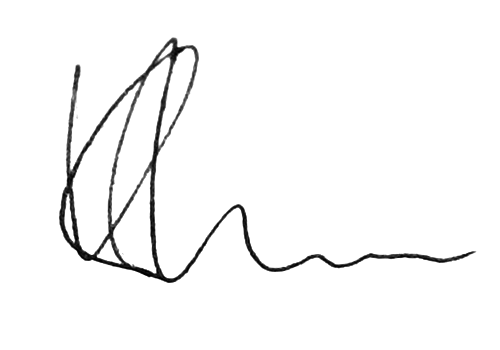
\includegraphics[scale=0.2]{../Resources/Signature/Kunal-Sig.png} \\
    
    Gabriel Castagner & Introduction, System Architecture, Analysis Class Diagram &
    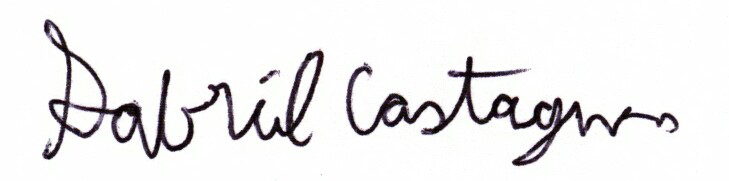
\includegraphics[scale=0.2]{../Resources/Signature/Gabe-Sig.png} \\
    
    Victor Velechovsky & Introduction & 
    
\includegraphics[scale=0.3]{../Resources/Signature/Vic-Sig.png} \\
    
    Josh Mitchell & Subsystems, CRC Cards & 
    
\includegraphics[scale=0.2]{../Resources/Signature/Josh-Sig.png} \\
\end{tabular}
% End Section



\end{document}
%------------------------------------------------------------------------------